\documentclass[
  american        % uncomment for english architecture
  %ngerman         % uncomment for german architecture
]{sirrixreport}

% -------------------------------------------------------------------
% Required Packages
% -------------------------------------------------------------------

\usepackage{svnkw}
\usepackage[
  % hideAnnotations    % Hides all annotations
  % hideCommentblock   % Hides all commentblock environments
]{sirrixcomments}
\usepackage{requirements}  % For software architecture documents
\usepackage{usecase}       % For software architecture documents
\usepackage{listings}

% -------------------------------------------------------------------
% The Title
% -------------------------------------------------------------------

% Headline
\heading{The Turaya Security Framework}
% An optional logo shown in the middle of the page. A project logo,
% or something similar.
 \logo{\includegraphics[width=9cm]{tpmmanager_cover} } %%%%%%%%%%%%%%%%%%%%%%%%%%%%<<<<<<<<<-------------------------<<<<<<<<%%%%%%%%%
% Title
\title{The TPM Manager}
\subtitle{Requirements, Design, and Implementation}
% Author or list of authors
%\author{Anoosheh Zaerin\\\url{a.zaerin@sirrix.com}}  % Use \and to add more authors...
%\and{Ren\'e Korthaus\\\url{r.korthaus@sirrix.com}}
% Current status, e.g., version number or date (\today)
\status{\today}
%\substatus{Revision~\svnkw{LastChangedRevision}} 

% -------------------------------------------------------------------
% Local Macros
% -------------------------------------------------------------------

% Required by the examples...
\newcommand{\System}{TPM Manager}  % Replace by product name or sth. similar

% -------------------------------------------------------------------
% The main part
% -------------------------------------------------------------------

\begin{document}

\maketitle		% The title page
\cleardoublepage        % 2nd page should be blank

% The default author page
\begin{table}
{\large \textbf{Author:}}\\

Anoosheh Zaerin\\
\url{a.zaerin@sirrix.com} \\
\\
Ren\'e Korthaus\\
\url{r.korthaus@sirrix.com} \\
\\
{\large \textbf{Advisors:}} \\

              Ahmad-Reza Sadeghi \\
             \url{ahmad.sadeghi@trust.rub.de} \\

 Christian Stueble \\
             \url{c.stueble@sirrix.com}

\end{table}



\tableofcontents	% ...
\listoffigures
%\listoftables

\lstloadlanguages{C++,C,bash}
\lstset{language=C++,
        basicstyle=\small,
   commentstyle=\itshape,
   identifierstyle=\ttfamily,
   keywordstyle=\ttfamily,
   stringstyle=\ttfamily
}

%%%%%%%%%%%%%%%%%%%%%%%%%%%%%%%Abstract und Keywords???????????????

%======================================================================
\chapter{Introduction}
\label{chap:usingclassfile}
%======================================================================

% ------------------------------------------------------------------------
%                       Motivation and Problem Description
% ------------------------------------------------------------------------
\section{Motivation and Problem Description}
\label{sec:motivation}

The computer industry has recently come up with Trusted Computing (TC), a new generation of computing platforms based on new architectures both in hardware and software. The results of their investigations are the \TCG initiative that has published the corresponding hardware and software specifications \cite{TPM_1.2.103}.
The basic idea is to embed elementary security functions into the underlying hardware of the computing platform while keeping the assumption on tamper-resistance as weak as possible, and reducing costs by keeping the trusted component as small as possible.

The stated goal of these architectures is to improve the security and trustworthiness of computing platforms. Indeed, these platforms offer many useful functions which can be used to increase a platform's security. They extend the conventional PC architecture by new mechanisms to (i) protect cryptographic keys, (ii) generate random numbers in hardware, (iii) authenticate (the configuration of) a platform (attestation), and (iv) cryptographically bind the data to be encrypted to certain information, e.g., the system configuration and the identifier of the invoking application (sealing). 

However, there is still an ongoing public debate about the negative economical, social, and technical consequences of these platforms. People are concerned about the potential dangers of the capabilities of such platforms: They may give vendors and content providers too much control power over personal systems and users' private information. Although most complains about trusted computing are speculative, it is highly important to observe its development carefully, and to improve this technology by putting together the missing pieces for more secure platforms in future. 
Today, only a few software components supporting TPMs are available, especially in the context of open-source operating systems like Linux. We observed that many people, who would like to experience with a \TPM, have many problems using the provided management software, i.e., libtpm and Trousers. Moreover, many open-source projects in the context of trusted computing lack support of a TPM management.

% ------------------------------------------------------------------------
\section{Goals}
The goal of ``TPM Manager`` project is the realization of an open source TPM management software providing an easy-to-use graphical user interface. Currently, the TPM Manager can be used under Linux, while later releases should also be usable as a compartment executed on top of a security kernel such as Turaya or OpenTC. Current releases of the TPM Manager were developed by Sirrix AG and Ruhr-University Bochum. The TPM Manager is published under version 2 of the GNU GPL license.

%======================================================================
\chapter{Requirements Specification}
\label{chap:requirements}
%======================================================================
This chapter defines the functional and supplementary requirements of the TPM Manager. It defines the target groups, roles and actors and gives an overview of use cases in \autoref{sec:overview}.


% ------------------------------------------------------------------------
\section{Target Groups}
 This section defines the users/other components that wish to use the product.

\begin{itemize}
 \item Home user (Single-user platform at home)
\end{itemize}

% ------------------------------------------------------------------------
%                       Roles and Actors
% ------------------------------------------------------------------------
\section{Roles and Actors}
 In this section we define different roles and actors important for the use case model. Actors are parties outside the system that interact with the system; an actor can be a class of users, roles users can play, or other systems. Note that, depending on the use case, some parties or actors may not be involved.

\begin{itemize}
 \item \emph{Owner:} The owner of a platform is an entity who defines the allowed configurations of the underlying platform. Note that this also includes certain changes to the platform's configuration.  In practice, these changes are patches/updates. The platform owner is also owner of the TPM and thus is aware of the owner authorization information. Typical examples are an enterprise represented by an administrator or an end-user owning a personal platform.
 \item \emph{User:} The user of a computing platform is an entity interacting with the platform under the platform's security policy. Examples are employees using enterprise-owned hardware. User and owner might also be identical, e.g., in an end-user environment.
\end{itemize}

% ------------------------------------------------------------------------
%                           Functional Requirements
% ------------------------------------------------------------------------
\section{Functional Requirements (Use Case Model)}
\label{sec:functional.requirements}

  Each use case focuses on describing how to achieve a single business
  goal or task. From a traditional software engineering perspective a
  use case describes just one feature of the system.  For most
  software projects this means that multiple, perhaps dozens, of use
  cases are needed to fully specify the new system.  The degree of
  formality of a particular software project and the stage of the
  project will influence the level of detail required in each use
  case.
 
  A use case defines the interactions between external actors and the
  system under consideration to accomplish a business goal. Actors are
  parties outside the system that interact with the system; an actor
  can be a class of users, roles users can play, or other systems.
 
  Use cases treat the system as a ``black box", and the interactions
  with the system, including system responses, are perceived as such
  from outside the system. This is a deliberate policy, because it
  simplifies the description of requirements, and avoids the trap of
  making assumptions about how this functionality will be
  accomplished.
 
  \noindent A use case should:
 
  \begin{itemize}
  \item describe a business task to serve a business goal
  \item have no implementation-specific language
  \item be at the appropriate level of detail
  \item be short enough to implement by one software developer in a
    single release.
 \end{itemize}

% ------------------------------------------------------------------------
%                       Overview
% ------------------------------------------------------------------------
\section{Use case overview} 
\label{sec:overview}
\autoref{overview} gives on overview of all use cases realized by the TPM Manager. The use cases are separated into different subsets:
\begin{itemize}
 \item \emph{Info:} Display information about the TPM that can be read without an authorization.
 \item \emph{Owner Settings:} Use cases related to TPM Owner management and SRK management issues.
 \item \emph{TPM Settings:} Use cases related to TPM state management.
 \item \emph{Advanced:} Critical use cases that may cause permanent changes to the TPM
 \item \emph{Misc:} Utility use cases like password dialogs or warning messages.
\end{itemize}

\begin{figure}[h]
 \centering
 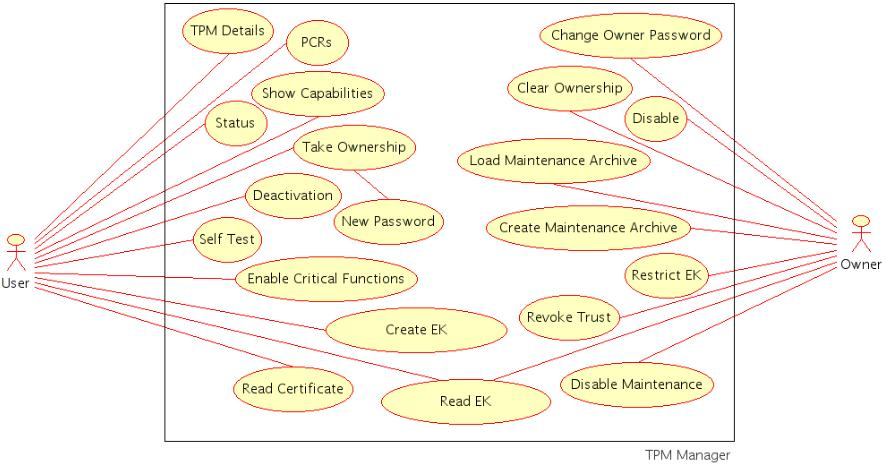
\includegraphics[width=1\textwidth]{images/all_functions.jpg}
 % graphic3.jpg: 994x517 pixel, 72dpi, 35.07x18.24 cm, bb=0 0 994 517
 \caption{Overview of all use cases realized by the TPM Manager.}
 \label{overview}
\end{figure}
\clearpage

% ------------------------------------------------------------------------
\subsection{Info}

The use cases described in this section display information about the TPM and can be read without authorization.

\begin{usecase}{Info}{info}
\ucdesc Show the status of the TPM.
\ucactors  User
\ucnormal 
 \item User clicks on the ''Info`` tab
 \item The following information will be displayed:
   \begin{compactitem}
   \item TPM enabled
   \item TPM activated
   \item TPM Owner set
   \item Endorsement Key available
   \item TPM driver found
   \item TSS system found
   \end{compactitem}
\ucendflow 
\end{usecase}


\begin{figure}[h]
\centering
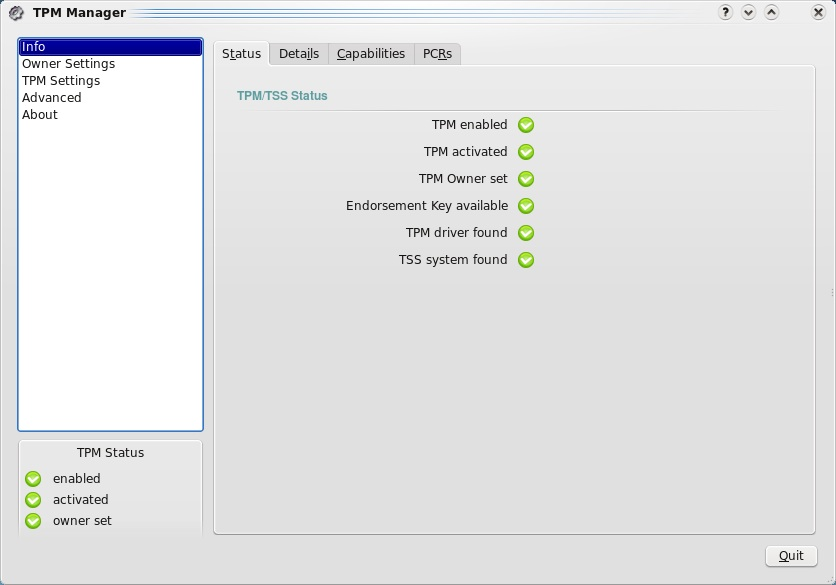
\includegraphics[width=0.8\textwidth]{images/uc10.jpg}
\caption{Overview of \ucref{info}.}
\end{figure}
\clearpage

\begin{usecase}{TPM Details}{details}
\ucdesc Show detailed information about the TPM and the TSS
\ucactors  User
\ucnormal 
 \item User clicks on the ''Details`` tab
 \item The following information will be displayed:
   \begin{compactitem}
   \item Information about TPM such as:
      \begin{compactitem}
         \item Vendor
         \item Version
         \item Firmware
      \end{compactitem}
   \item Information about TSS such as:
      \begin{compactitem}
         \item Vendor
         \item Version
      \end{compactitem}
   \end{compactitem}
\ucendflow 
\end{usecase}

\begin{figure}[h]
\centering
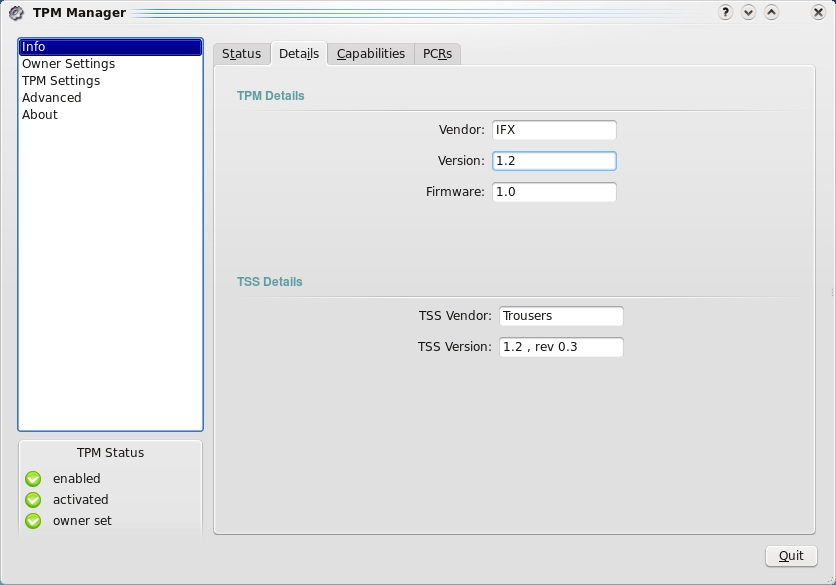
\includegraphics[width=0.8\textwidth]{images/uc20.jpg}
% graphic4.jpg: 751x445 pixel, 762dpi, 2.50x1.48 cm, bb=0 0 71 42
\caption{TPM and TSS details tab dialog \ucref{details}} 
\end{figure}
\clearpage

\begin{usecase}{Show TPM Capabilities}{capability}
\ucdesc Show the capabilities of the TPM
\ucactors  User
\ucnormal 
 \item User clicks on the ''Capability`` tab
 \item The following information will be displayed:
   \begin{compactitem}
   \item Number of PCRs
   \item Number of keys that can be loaded into TPM
   \item Available features
   \item etc.
   \end{compactitem}
\ucendflow 
\end{usecase}

\begin{figure}[h]
\centering
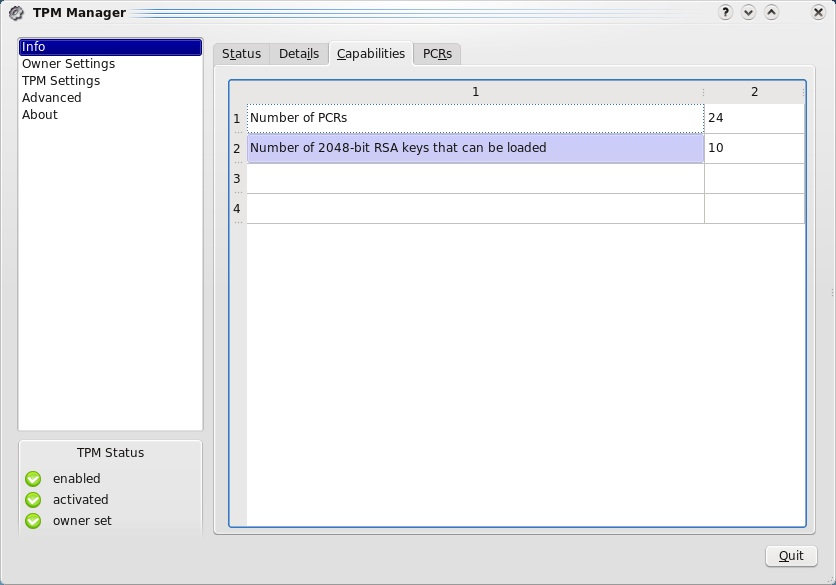
\includegraphics[width=0.8\textwidth]{images/uc30.jpg}
% graphic4.jpg: 751x445 pixel, 762dpi, 2.50x1.48 cm, bb=0 0 71 42
\caption{Dialog showing the capabilities supported by the TPM \ucref{capability}.} 
\end{figure}
\clearpage


\begin{usecase}{PCRs}{pcrs}
\ucdesc Show the current PCR values.
\ucactors  User
\ucnormal 
 \item User clicks on the ''PCRs`` tab
 \item Display current PCR values
\ucendflow 
\end{usecase}

\begin{figure}[h]
 \centering
 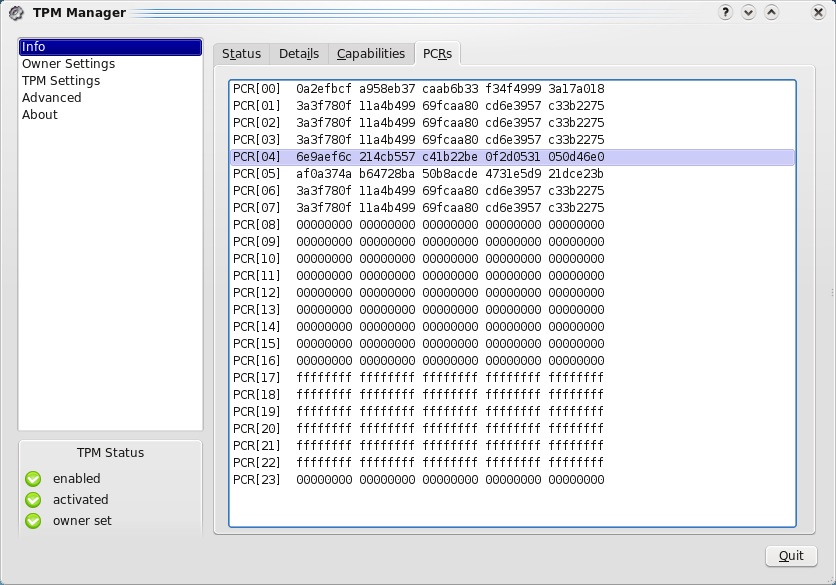
\includegraphics[width=0.8\textwidth]{images/uc40.jpg}
% graphic6.jpg: 713x421 pixel, 762dpi, 2.38x1.40 cm, bb=0 0 67 40
 \caption{PCR value dialog \ucref{pcrs}}
\end{figure}
\clearpage

% ----------------------------------------------------------------------
\subsection{Owner Settings}
The use cases of this section are related to TPM Owner management and \SRK management issues.

\begin{usecase}{Take Ownership}{takeowner}
\ucdesc Configure the Owner and set the embedded Security features
\ucactors Owner
\ucinclude New Password
\ucprecond No TPM owner set
\ucpostcond TPM Owner set
\ucnormal 
 \item User clicks on the ''Ownership`` tab
 \item User hits the ''Take`` button
 \item TPM Manager displays a dialog to choose the owner password
 \item User chooses the owner password and confirms it
 \item TPM Manager displays a dialog to choose the type of SRK password
 \item User chooses the default choice (set SRK password to \lstinline'WELL_KNOWN_SECRET')
 \item TPM Manager sets SRK password to \lstinline'WELL_KNOWN_SECRET'
 \item TPM Manager sets the owner and SRK password and displays a dialog whether the passwords were successfully set or not
\ucendflow 
\ucalternate
 \item User clicks on the ''Ownership`` tab
 \item User hits the ''Take`` button
 \item TPM Manager displays a dialog to choose the owner password
 \item User chooses the owner password and confirms it
 \item TPM Manager displays a dialog to choose the type of SRK password
 \item User chooses the second choice (set SRK password manually)
 \item TPM Manager displays a dialog to choose the SRK password
 \item User chooses SRK password and confirms it
 \item TPM Manager sets the password and displays a dialog whether the owner and SRK password were successfully set or not
\ucendflow 
\end{usecase}
\clearpage

\begin{usecase}{Change Owner Password}{changeowner}
\ucdesc Change the password used to authenticate the TPM owner
\ucactors Owner
\ucinclude 
   \begin{compactitem}
      \item Owner authentication \ucref{ownerauth}
      \item New Password \ucref{newpass}
   \end{compactitem}
\ucprecond TPM owner set
\ucpostcond New password for TPM Owner
\ucnormal 
 \item User clicks on the ''Ownership`` tab
 \item User hits the ''Change`` button
 \item TPM Manager displays a dialog window asking for current owner password
 \item TPM Owner types the current owner password
 \item TPM Manager displays dialog asking for new owner password
 \item TPM Owner types new owner password
 \item TPM Manager sets the new owner password and displays a dialog whether the new owner password was successfully set or not
\ucendflow 
\end{usecase}
\clearpage

\begin{usecase}{Clear Ownership}{clearowner}
\ucdesc Delete the TPM ownership and set TPM to factory defaults
\ucactors Owner
\ucinclude 
         \begin{compactitem}
            \item Owner authentication \ucref{ownerauth}
            \item Warning \ucref{warning}
         \end{compactitem}
\ucprecond TPM owner set
\ucpostcond TPM Disabled, Deactivated, and no Owner set
\ucnormal
 \item User clicks on the ''Ownership`` tab
 \item User hits the ''Clear`` button
 \item TPM Manager displays a dialog window asking for owner password
 \item TPM owner types the owner password
 \item TPM Manager checks the owner password and clears the TPM
 \item TPM Manager displays a dialog whether the TPM was successfully cleared or not
\ucendflow 
\end{usecase}

\begin{figure}[h]
 \centering
 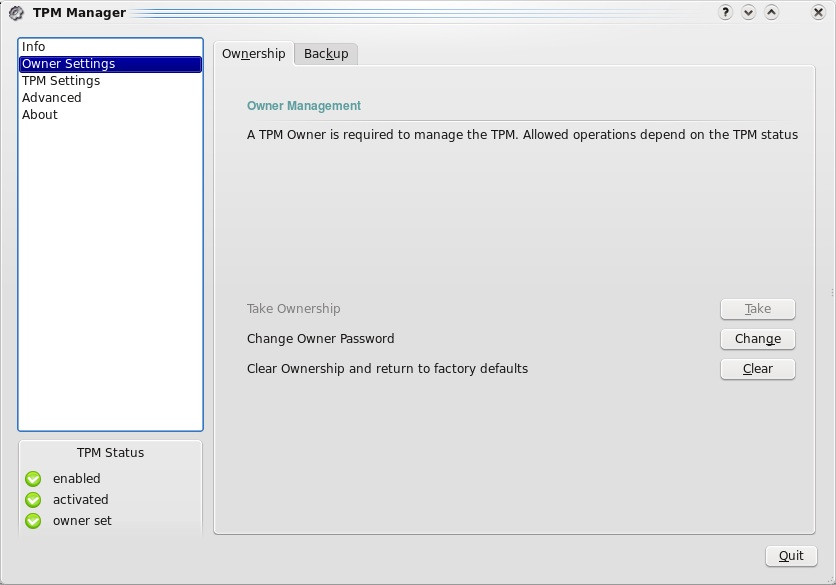
\includegraphics[width=0.8\textwidth]{images/uc_owner.jpg}
 \caption{''Ownership`` tab Dialog \ucref{takeowner}, \ucref{changeowner} and \ucref{clearowner}}
\end{figure}
\clearpage


\begin{usecase}{Create Maintenance Archive}{maintenance}
\ucdesc Create a backup of the SRK
\ucactors  Owner
\ucinclude 
   \begin{compactitem}
      \item File selection
      \item Owner authorization
   \end{compactitem}
\ucprecond TPM supports maintenance feature
\ucnormal 
 \item Owner hits ``Create'' maintenance button
 \item Owner selects destination for archive file
 \item TPM Manager asks for owner authorization
 \item Owner confirms creation 
\ucendflow
\end{usecase}
\clearpage

\begin{usecase}{Load Maintenance Archive}{loadmaintenance}
\ucdesc Restore the SRK backup archive
\ucactors  Owner
\ucinclude 
   \begin{compactitem}
      \item File selection
      \item Owner authorization
   \end{compactitem}
\ucprecond SRK archive was created by the TPM manufacturer
\ucnormal 
 \item Owner hits ``Load'' maintenance button
 \item Owner selects maintenance archive file
 \item TPM Manager asks for owner authorization
 \item Owner confirms loading maintenance archive
\ucendflow
\end{usecase}

\begin{figure}[h]
 \centering
 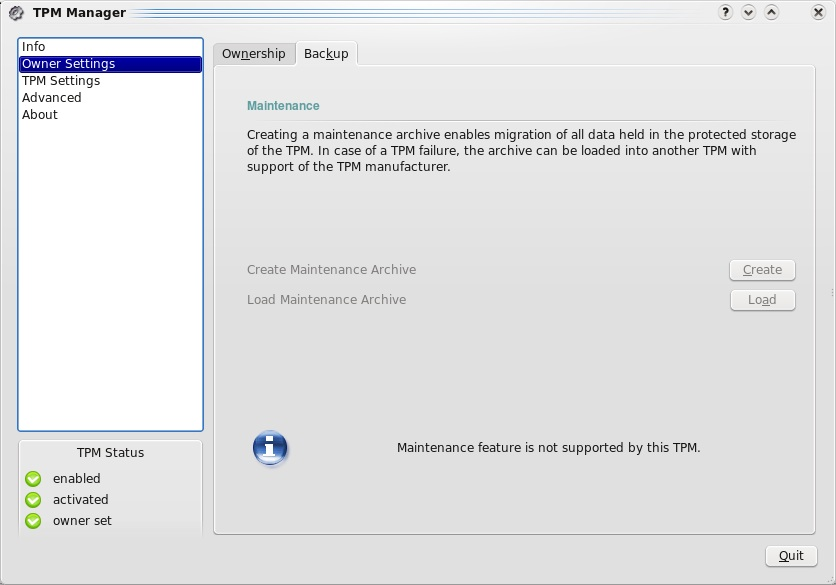
\includegraphics[width=0.8\textwidth]{images/uc8090.jpg}
 \caption{''Maintenance`` tab dialog \ucref{maintenance}, \ucref{loadmaintenance}}
\end{figure}
\clearpage

% ------------------------------------------------------------------------
\subsection{TPM Settings}

\begin{usecase}{TPM Deactivation}{deactivate}
\ucdesc TPM can be switched from activated to temporarily deactivated mode
\ucactors  User %Operator
\ucprecond TPM is activated
\ucpostcond TPM is temporarely deactivated
\ucnormal 
 \item User hits ''Deactivate'' button
 %\item TPM Manager asks for operator authorization
 \item TPM Manager displays warning message
 \item TPM Manager displays dialog whether TPM was successfully deactivated or not
\ucendflow
\end{usecase}
Note: On 1.2 TPMs, temporarily deactivating the TPM requires operator authorization. When trying to deactivate a TPM 1.2 without operator authorization, a ''bad physical presence'' exception is thrown.

\clearpage

\begin{usecase}{Disable (Enable) the TPM}{disable}
\ucdesc TPM can be switched to enabled or disabled mode
\ucactors  Owner
\ucinclude 
   \begin{compactitem}
      \item Owner Authorization \ucref{ownerauth}
      \item Warning \ucref{warning}
   \end{compactitem}
\ucnormal 
 \item Owner hits ``Disable`` (``Enable``) button
 \item TPM Manager asks for owner authorization
 \item TPM Manager displays a warning message
 \item TPM Manager displays dialog whether TPM was successfully disabled (enabled) or not
\ucendflow
\end{usecase}

\begin{figure}[h]
 \centering
 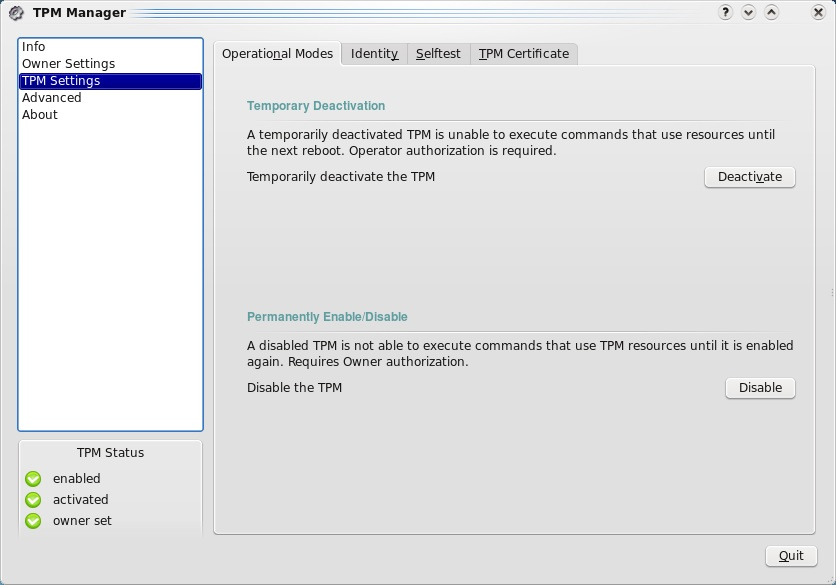
\includegraphics[width=0.8\textwidth]{images/uc100110.jpg}
 \caption{TPM operational modes dialog. Implements \ucref{deactivate} and \ucref{disable}}
\end{figure}
\clearpage


\begin{usecase}{Create Endorsement Key}{createek}
\ucdesc Create Endorsement Key
\ucactors  User
\ucinclude 
   \begin{compactitem}
      \item Owner Authorization \ucref{ownerauth}
      \item Warning \ucref{warning}
   \end{compactitem}
\ucprecond No Endorsement Key is set by manufacturer
\ucpostcond TPM has Endorsement Key
\end{usecase}


\begin{usecase}{Read Public Endorsement Key}{readek}
\uctitle Read the public part of EK
\ucactors  User
\end{usecase}

\begin{usecase}{Store Public Endorsement Key}{readek}
\uctitle Store the public part of EK outside the TPM
\ucactors  User
\end{usecase}

\begin{usecase}{Restrict Public Endorsement Key}{restrictedek}
\ucdesc Disable reading of EK without owner authorization
\ucactors  Owner
\ucinclude
  \begin{compactitem}
      \item Owner Authorization \ucref{ownerauth}
      \item Warning \ucref{warning}
   \end{compactitem}
\ucprecond 
   \begin{compactitem}
      \item Owner set
      \item Endorsement Key is not restricted
   \end{compactitem}
\ucpostcond Need owner authentication to read Endorsement Key
\end{usecase}
\clearpage

\begin{usecase}{Read TPM Endorsementcertificate}{readekcert}
\ucdesc Read the Endorsement Certificate of the TPM
\ucactors  User
\end{usecase}

\begin{figure}[h]
 \centering
 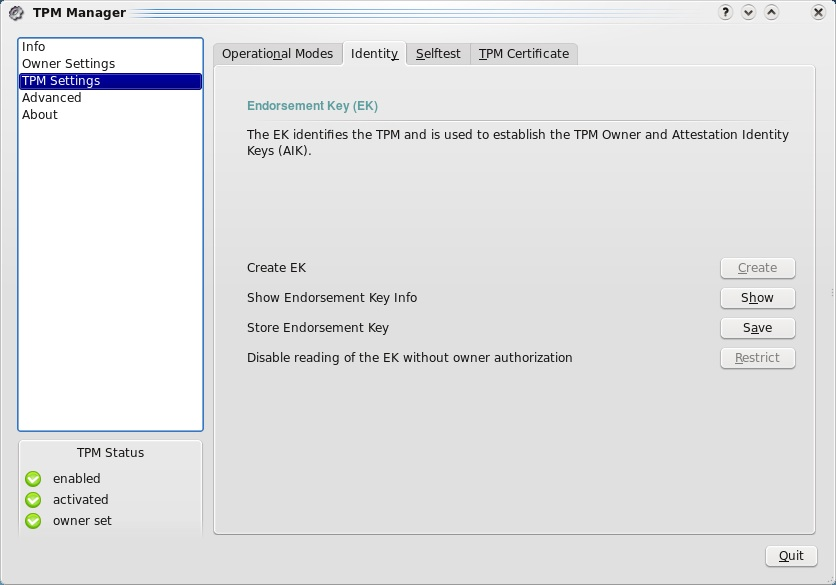
\includegraphics[width=0.8\textwidth]{images/uc_identity.jpg}
 \caption{''Endorsement`` tab dialog \ucref{createek}, \ucref{readek}, \ucref{restrictedek} and \ucref{readekcert}}
\end{figure}
\clearpage

\begin{usecase}{Self test}{selftest}
\ucdesc Perform a full self test of each TPM internal function
\ucactors  User
\end{usecase}

\begin{figure}[h]
 \centering
 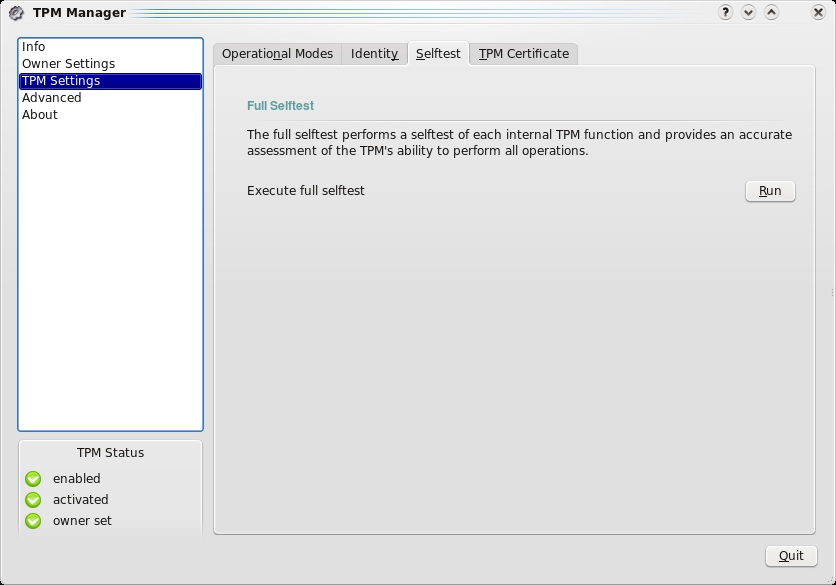
\includegraphics[width=0.8\textwidth]{images/uc_selftest.jpg}
 \caption{Tab dialog to perform a full TPM self test \ucref{selftest}}
\end{figure}
\clearpage

\begin{usecase}{Show TPM Certificate}{certificate}
\ucdesc Shows the TPMs manufacturer certificate is present
\ucactors  User
\end{usecase}

\begin{figure}[h]
 \centering
 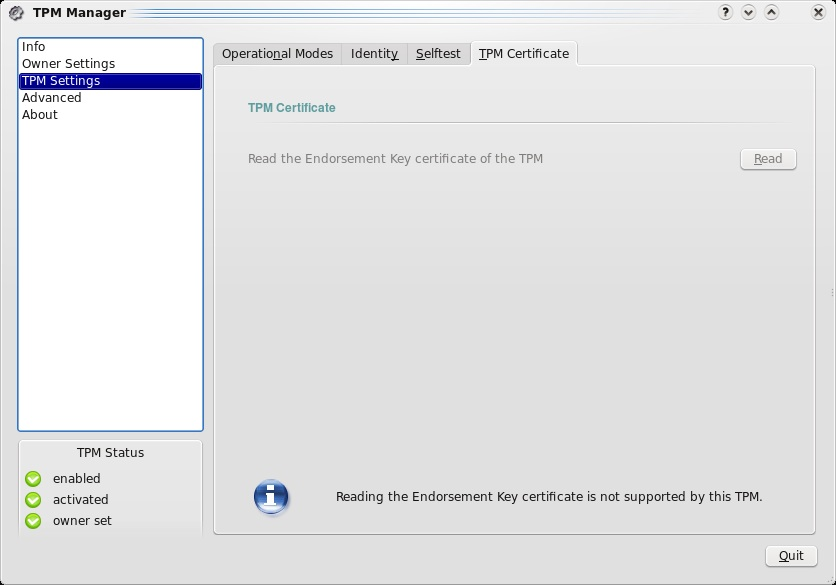
\includegraphics[width=0.8\textwidth]{images/uc_tpmcert.jpg}
 \caption{Tab dialog to show the TPM certificate \ucref{certificate}}
\end{figure}
\clearpage


% ------------------------------------------------------------------------
\subsection{Advanced}

\begin{usecase}{Warning Critical Functions}{critical}
\ucdesc The ''Advanced'' section warns the user about criticality of the features provided, because these features can do permanent changes to the TPM
\ucactors Owner
\end{usecase}

\begin{figure}[h]
 \centering
 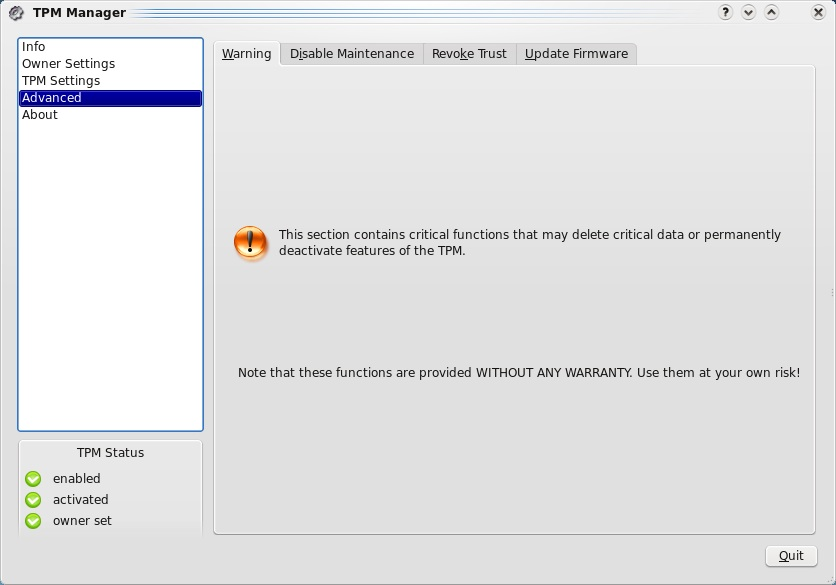
\includegraphics[width=0.8\textwidth]{images/uc_advanced_warning.jpg}
 \caption{Tab dialog warning about critical features \ucref{critical}}
\end{figure}
\clearpage


\begin{usecase}{Disable Maintenance Feature}{disablemain}
\ucdesc Kills Maintenance feature
\ucactors Owner
\ucinclude Owner authorization
\end{usecase}

\begin{figure}[h]
 \centering
 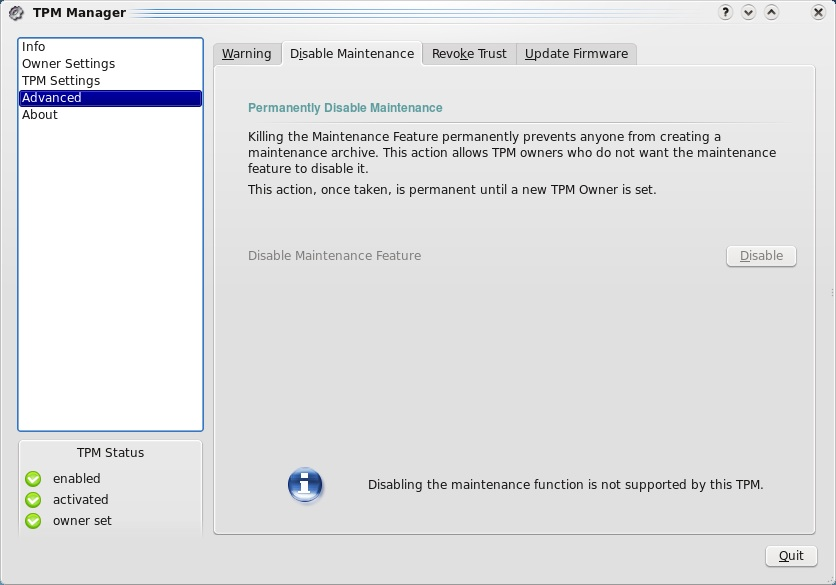
\includegraphics[width=0.8\textwidth]{images/uc_disable_maint.jpg}
 \caption{Disable Maintenance \ucref{disablemain}}
\end{figure}
\clearpage

\begin{usecase}{Revoke Trust}{revoke}
\ucdesc Delete Endorsement Key
\ucactors  Owner
\ucinclude 
   \begin{compactitem}
      \item Owner Authorization \ucref{ownerauth}
      \item Warning \ucref{warning}
   \end{compactitem}
\ucprecond TPM has Endorsement Key
\ucpostcond TPM has no Endorsement Key
\end{usecase}

\begin{figure}[h]
 \centering
 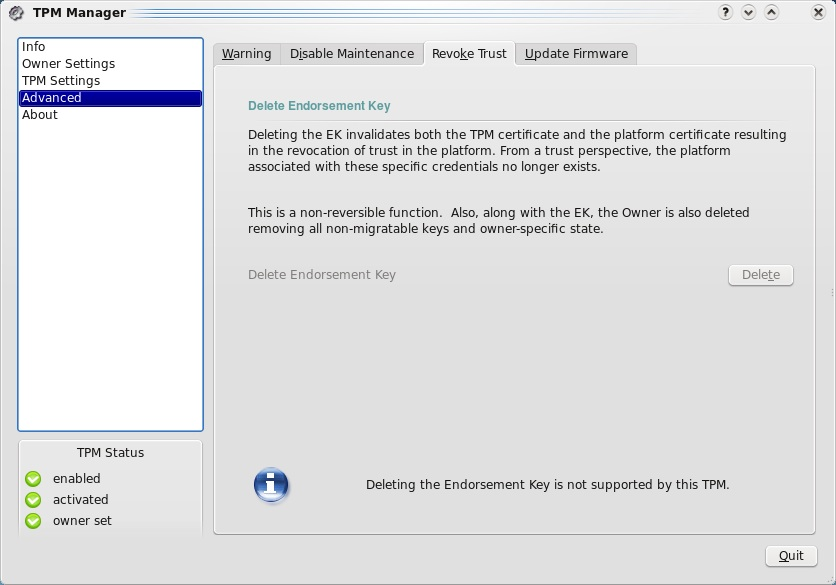
\includegraphics[width=0.8\textwidth]{images/uc_revoketrust.jpg}
 \caption{``Revoke Trust'' tab dialog \ucref{revoke}}
\end{figure}
\clearpage

% ------------------------------------------------------------------------
\subsection{Misc.}
The uses cases of this section include utility dialogs like password dialogs or warning messages.

\begin{usecase}{New Password}{newpass}
\ucdesc User/Owner enters a new passphrase
\ucactors  Owner, User
\end{usecase}

\begin{usecase}{Owner Authentication}{ownerauth}
\ucdesc Owner authorization using the owner secret
\ucactors  Owner
\end{usecase}

\begin{usecase}{Warning Message}{warning}
\ucdesc System shows a warning message
\ucactors  Owner, User
\end{usecase}
\clearpage

% ------------------------------------------------------------------------
%                         Supplementary Requirements
% ------------------------------------------------------------------------
\section{Supplementary Requirements}

This section describes obligatory criteria, mandatory for successful completion.

%-------------------------------------------------------------------------
\subsection{Preconditions}


Requirements that have to be fulfilled already, because they were
 needed for the development process are descriebd in this section.

\prerequisite{100}{TSS}
The TPM Manager will depend on an existing \TSS implementation.

\prerequisite{200}{Widget Library}
The TPM Manager will depend on an open-source widget library.

\prerequisite{300} {TPM-enabled BIOS}
The BIOS has to support the TPM to be able to enable it.

%------------------------------------------------------------------------
\subsection{Required Criteria}

Mandatory criteria, that are obligatory for successful completion are descriebd in this section.

\mandatory{10}{Linux support}
The realization of the use cases should be based on an Linux-based architecture.


%-----------------------------------------------------------------------
\subsection{Desired Criteria}

  Optional criteria, that are not mandatory for successful completion are descriebd in this section.

\desired{10} {Turaya support} 
The realization of the use cases should be based on a Turaya-based architecture.

% ----------------------------------------------------------------------
\subsection{Execution Environment}

   This section specifies software and hardware the user requires at
   least to run our product successfully.


\subsubsection{Software}
\label{subsec:software}
\begin{compactitem}
 \item (required) Linux Distribution based on kernel 2.6.x, including
   \begin{compactitem}
      \item TrouSerS-TSS
      \item TPM Driver
      \item Widget Library
   \end{compactitem}
 \item (optional) Turaya Architecture, including
   \begin{compactitem}
      \item TPM Driver
      \item Widget Library
      \item Trust Manager
   \end{compactitem}
\end{compactitem}

\subsubsection{Hardware}
\begin{compactitem}
 \item HP Notebook with Infineon TPM 1.1.b
 \item HP Notebook with Infineon TPM 1.2
 \item Desktop PC with ST TPM 1.2
 \item ThinkPad T41p with Atmel TPM 1.1b
\end{compactitem}

% ---------------------------------------------------------------------
\subsection{Development Environment}

   This section specifies hard- and software that developers need at
   least to implement the product successfully.

% ------------------------------------------------------------------------
\subsection{Software}
\begin{compactitem}
 \item Linux 2.6.x
 \item g++ 4.3.x
 \item Qt4 Libraries 4.4.x
 \item QDevelop
 \item Qt4 Designer
\end{compactitem}

% ------------------------------------------------------------------------
\subsection{Hardware}
\begin{compactitem}
 \item HP Notebook
 \item TPM 1.1b
 \item TPM 1.2
\end{compactitem}

%======================================================================
\chapter{Software Architecture}
\label{chap:architecture}
%======================================================================

% ------------------------------------------------------------------------
%                       Introduction
% ------------------------------------------------------------------------
\section{Introduction}
This chapter provides an overview of the TPM Manager's design.
In \autoref{sec:logicalview} the architecturally significant parts of the  design model are described, and \autoref{sec:usecase} 
illustrates how the TPM Manager actually works by giving a few selected use-case realizations, and explains how the various design 
model elements contribute to their functionality.


% ------------------------------------------------------------------------
%                       Logical View
% ------------------------------------------------------------------------
\section{Logical View} 
\label{sec:logicalview}

This section describes the architecturally significant parts of the
design model, such as its decomposition into subsystems and
packages. And for each significant package, its decomposition into
classes and class utilities is illustrated. 

\begin{figure}[h]
 \centering
 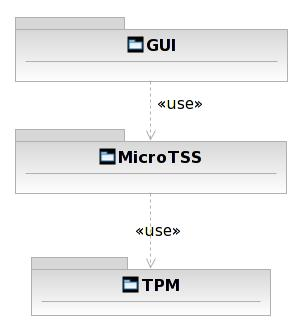
\includegraphics[width=0.4\textwidth]{images/tpmmanager_layers.jpg}
 \caption{The two layers of the TPM Manager design}
 \label{highleveldesign}
\end{figure}
\clearpage

\subsection{Overview}
This subsection describes the overall decomposition of the design model in terms of
its package hierarchy and layers. 


As illustrated in \autoref{highleveldesign}, the design of the TPM Manager has two layers, the \GUI layer and the MicroTSS layer.
While the GUI layer provides the user interface components, based on widgets of Qt\footnote{http://www.qtsoftware.com/} framework, the MicroTSS layer offers a simple, object-oriented interface to the functions
of the underlying TPM.


Although the current implementation of the MicroTSS is based on the TrouSerS TSS, the abstraction provided by the MicroTSS layer allows support from alternative
TSS implementations offered by a third party or from the required functions implemented directly.
The latter is especially important if the TPM Manager should be used in a security-critical
environment, e.g., as a part of a security kernel.


\subsection{Architecturally Significant Design Packages}


\paragraph{The GUI layer.}
The GUI layer of the TPM Manager offers an interface to the user and uses
the MicroTSS layer to access TPM functions. The logic of the user interface layer is realized by
the Qt-based class, \lstinline'TPM_Manager'. Its base class, \lstinline'TPM_ManagerBase', is created by the
Qt Designer, Trolltech's tool for designing and building GUI's. The
Qt Designer allows the addition of new functionality without much effort. \autoref{ownership} shows an
example screenshot of the TPM Manager GUI in use.

\begin{figure}[h]
 \centering
 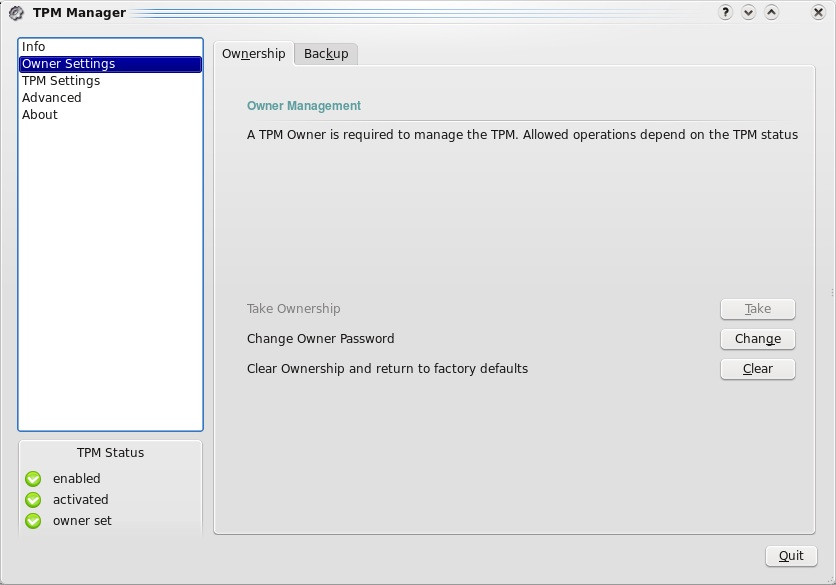
\includegraphics[width=0.8\textwidth]{images/uc_owner.jpg}
 \caption{``Ownership'' tab Dialog}
 \label{ownership}
\end{figure}
\clearpage

\paragraph{The MicroTSS layer.} The MicroTSS layer provides an abstract interface to access the TPM
and hides implementation details. \autoref{fig:interface} shows the \UML model
of the public interfaces and components provided by the TPM Manager and the \TSPI. The main component is the class \lstinline'TPM' that implements the TPM management
functions. The class \lstinline'TPM' is created by the class \lstinline'TSS' managing access to the TSS implementation in
use. For example, the class \lstinline'TSS' checks the availability of a TPM driver before creating an object
of type \lstinline'TPM'. The class \lstinline'PublicKey' provides information about types and attributes of cryptographic
encryption and test keys managed by the \lstinline'TSS'. Although the MicroTSS interface includes a small
number of functions related to version 1.2 of the TSS specification\cite{TSS_1.2}, the main portion is based on
TrouSerS TSS version 1.1b\cite{TSS_1.1}.


The current implementation of the class \lstinline'TPM' itself uses the TSPI interface provided by the \lstinline'libtspi.so'
library of TrouSerS. Since the TSPI interface includes many functions, in \autoref{fig:interface}, only the 
functions that are required to realize the use case ``Take Ownership'' are described in \autoref{sec:takeowner}.

\begin{figure}[h]
 \centering
 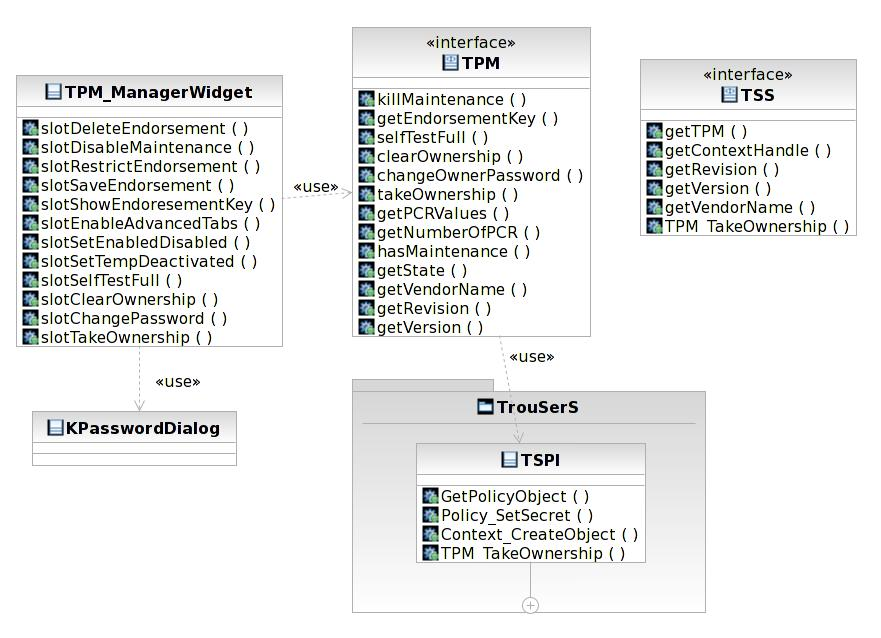
\includegraphics[width=0.8\textwidth]{images/tpmmanager_interfaces.jpg}
 \caption{Interfaces provided and used by the TPM Manager and the MicroTSS}
 \label{fig:interface}
\end{figure}
\clearpage

\section{Use Case Realization} 
\label{sec:usecase}
To illustrate the dynamic behavior of the TPM Manager design packages, the use cases ``Take Ownership'', ``Enable/Disable`` the TPM and ''PCRs`` are
explained in the following.

\subsection{Use Case Take Ownership}
\label{sec:takeowner}
The sequence diagram illustrated in \autoref{ownershipflow} describes the message and
control flow upon invocation of the ``Take Ownership'' function in the TPM Manager.

After the user presses the appropriate button of the TPM Manager dialog, the method \lstinline'slotTakeOwnership'()
of the class \lstinline'TPM_Manager' is invoked (step 1). Here, two password dialogs are created for entering
the TPM owner password and the SRK passoword (steps 1.1 and 1.3). Next, the MicroTSS,
more concretely the method \lstinline'takeOwnership'() of the class \lstinline'TPM', is invoked (step 1.5). This method
hides the complexity of the interface of the \lstinline'libtspi.so' by invoking \lstinline'TSPI' functions by setting the owner password and the \lstinline'SRK' password to finally take ownership of the TPM (steps 1.5.1 to 1.5.11). Lastly, a dialog informs the user about the result 
of the take ownership operation (step 1.7).

\begin{figure}[h]
 \centering
 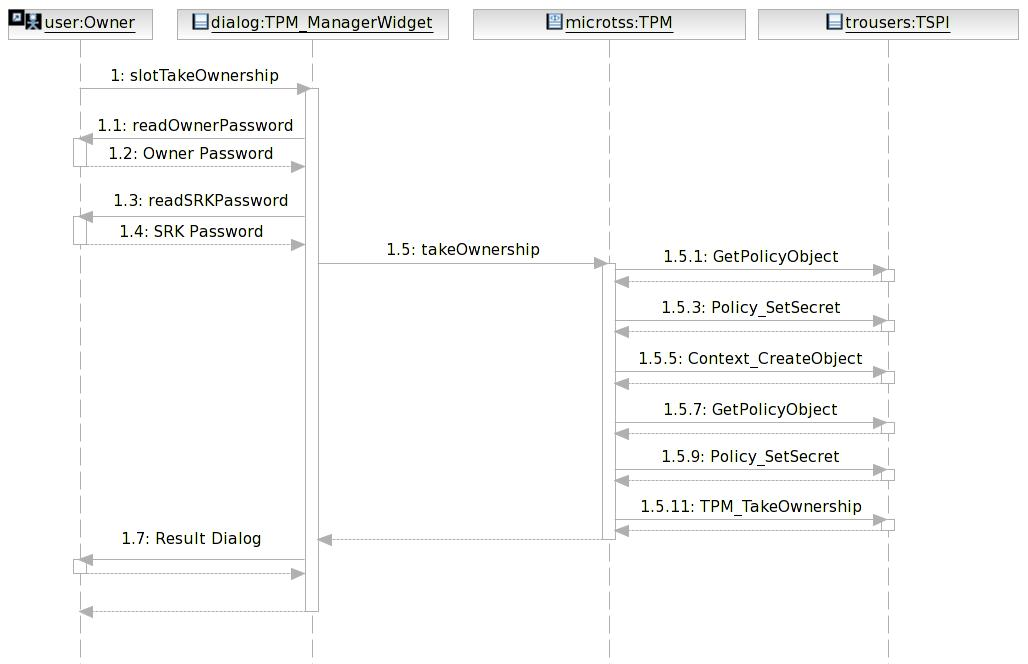
\includegraphics[width=0.9\textwidth]{images/uc50_flow.jpg}
 \caption{Control flow for ``Take Ownership`` function in the TPM Manager}
 \label{ownershipflow}
\end{figure}
\clearpage

\subsection{Use Case Enable/Disable}
The ''Enable``/''Disable`` button on the ''Operational Mode`` page of the TPM Manager GUI will be only active if the ownership of the TPM is done successfully. The caption of the button is set by class \lstinline'TPM_Manager' correspondence to the current status of the TPM. If the TPM is enabled the button is set to Disable and if the TPM is disabled the caption of the button will be Enable.

After the user clicks on the ''Enable``/''Disable`` button on the TPM Manager dialog, the appropriate method \lstinline'slotSetEnabledDisabled()' of the class \lstinline'TPM_Manager' is called. This method invokes a password dialog that asks for owner password. After the correct owner password is given by the user, the appropriate funtions \lstinline'setDisabled()'/\lstinline'setEnabled()' will be called, that are methods of the class \lstinline'TPM'. Lastly, a dialog informs the user about the result of the Enable/Disable operation.

\subsection{Use Case PCRs}
Choosing ''Info'' option from the left menu and then choosing the ``PCRs'' tab the function of \lstinline'TPM_Manager' will be called. It shows the current values of the PCRs only if the TPM is activated. The values are regularely updated by a signal coming from the system timer every 1 second. 

%======================================================================
\chapter{User Manual}
%======================================================================

% ------------------------------------------------------------------------
%                       Installation and Configuration
% ------------------------------------------------------------------------
\section{Requirements}
Since the TPM Manager is based entirely on the Qt UI framework, corresponding header and library files Qt4 should be in the library path. On some linux distributions you have to install the developer version of Qt to have the header files used by TPM Manager.

The required programs to install the TPM Manager are: 
\begin{itemize}
   \item Qt4
   \item TrouSerS
\end{itemize}

The required packages for (k)ubuntu in detail are:
\begin{itemize}
   \item build-essential
   \item libtspi-dev
   \item libtspi1
   \item trousers
   \item libqt4-dev
\end{itemize}

To use the features of the TPM Manager you need a running TrouSerS daemon.
The TPM Manager has been successfully compiled under Qt version 4.4.3 and KDE 4.1 respectively GNOME 2.26.


\section{Installation and Configuration}
The TPM Manager is hosted on sourceforge at \url{http://sourceforge.net/projects/tpmmanager/}. The software is based on qmake; therefore, it can be configured and installed as described below. Note that on some systems, qmake points to an older version of Qt - Qt3. Check your version of Qt prior to compiling TPM Manager as described below.


 \begin{lstlisting}[caption=Configuring and compiling the TPM Manager:, frame=lines]
 # tar -xzf tpmmanager-0.6.tar.gz
 # cd tpmmanager-0.6
 # qmake --version
 # qmake // if qmake --version returns Qt version 3.x.x, use qmake-qt4 instead
 # make
 # make install
 \end{lstlisting}  


% ------------------------------------------------------------------------
%                       Usage
% ------------------------------------------------------------------------
\clearpage
\section{Usage}

After successfully installing the TPM Manager you can run the executable on the shell by call \texttt{tpmmanager} or you may choose it from your system application menu. 

\subsection{Overview}
As illustrated in \autoref{fig:tpmmanager} there are 3 parts in the TPM Manager GUI. 
Part 1 is mainly used as a list to select functional areas of the TPM Manager. Clicking on the items as ``Info'', ``Owner Settings'', etc. changes the view of Part 2. Part 2 is itself separated into different tabs. Each tab contains a group of functionality. Part 3 shows the current status of the TPM. \autoref{fig:stat1} shows on the left side the status of a TPM with no owner and on the right side the status of a disabled TPM and no owner is set.

\begin{figure}[h]
 \centering
   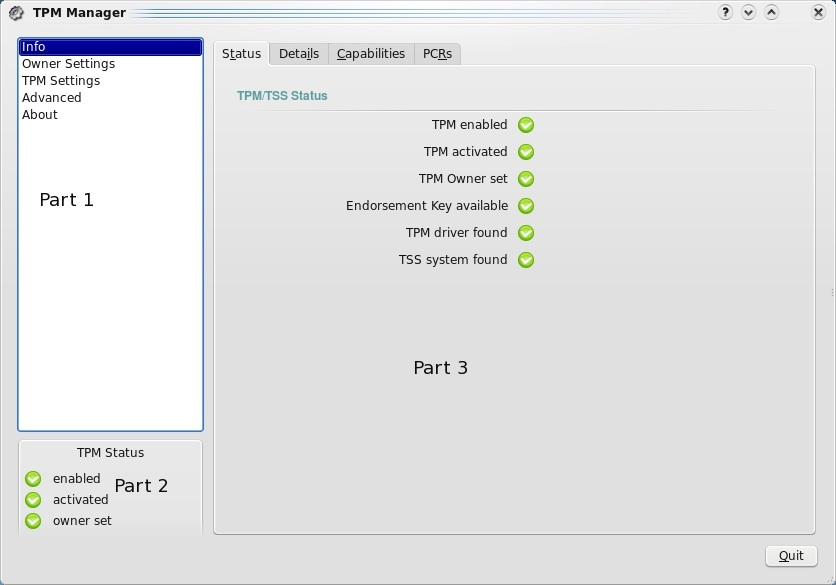
\includegraphics[width=0.8\textwidth]{images/tpmmanager_parts.jpg}
   \caption{3 parts of TPM Manager GUI}
\label{fig:tpmmanager}
\end{figure}
\begin{figure}[h]
 \centering
   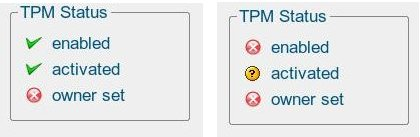
\includegraphics[width=0.5\textwidth]{images/stat.jpg}\caption{Status of the TPM}\label{fig:stat1}
\label{fig:stat2}
\end{figure}
\clearpage

\subsection{Info} This functional area provides some general information about the TPM and its status.
\subsubsection{Status tab} The ``Status'' tab gives some general information about the status of the TPM.
It shows also implicitly if you have a TPM chip on your system, by checking whether the TPM driver is loaded or not. \autoref{fig:status} shows the ''Status`` tab when a TPM driver but no TSS was found. \autoref{fig:status3} shows the ''Status'' tab when the TPM is disabled and no owner is set.
\begin{figure}[h]
 \centering
   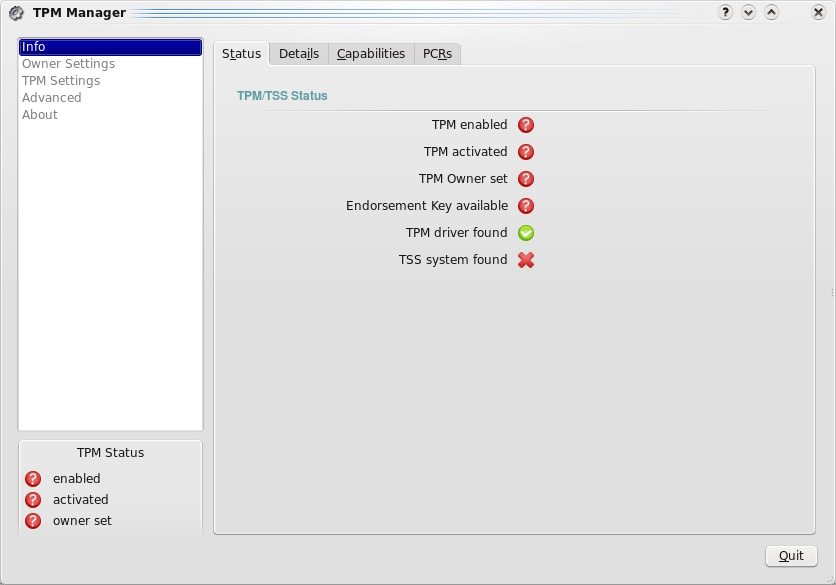
\includegraphics[width=0.8\textwidth]{images/tpmmanager_notss.jpg}
   \caption{Status of the TPM with no running TrouSerS}
\label{fig:status}
\end{figure}
\begin{figure}[h]
 \centering
   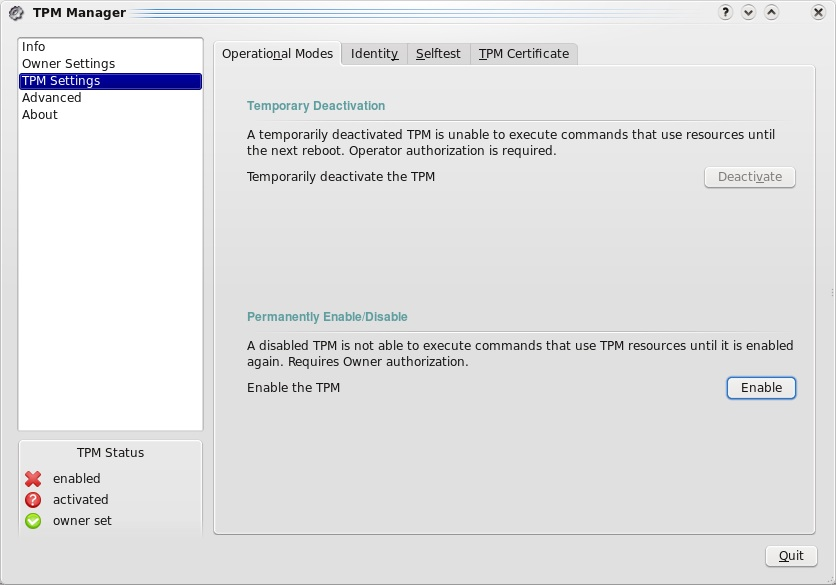
\includegraphics[width=0.8\textwidth]{images/tpmmanager_disabled.jpg}
   \caption{Status of the a disabled TPM}
\label{fig:status3}
\end{figure}
\clearpage

\subsubsection{Details tab} This page provides some information about the TPM version, the TPM vendor and also that of the TSS.

\subsubsection{Capabilities tab} This page shows values of some TPM capabilities.

\subsubsection{PCRs tab} This page shows the current values of all PCRs. The values are refresh every 1 second.

\subsection{Owner Settings} This functional area provides an interface to manage and backup the ownership of the TPM, as discussed in the following sections. 

\subsubsection{Ownership tab} This page gives you the possibility to manage the ownership of your TPM.

You can take the ownership of your TPM using the TPM Manager doing the steps described as follows.
\begin{itemize}
   \item Make sure that your TPM is enabled in the BIOS (See \autoref{fig:take}).
   \item Choose the ''Owner Settings'' from the left menu, and click on the ``Take'' button.
   \item Then choose a SRK password and confirm it, or choose the default password specified by TCG (WELL\_KNOWN\_SECRET) (See \autoref{fig:srk}).
   \item On the second dialog choose the owner password and confirm it. 
   \item Finally the TPM Manager will inform you whether taking ownership of the TPM was successfully or not(See \autoref{fig:take2}).
\end{itemize}
After doing a take ownership successfully you can use the ``Change'' button of the ``Ownership'' tab to change the owner password. You can also clear the owner using the ``Clear'' button on the same page.
\begin{figure}[h]
 \centering
   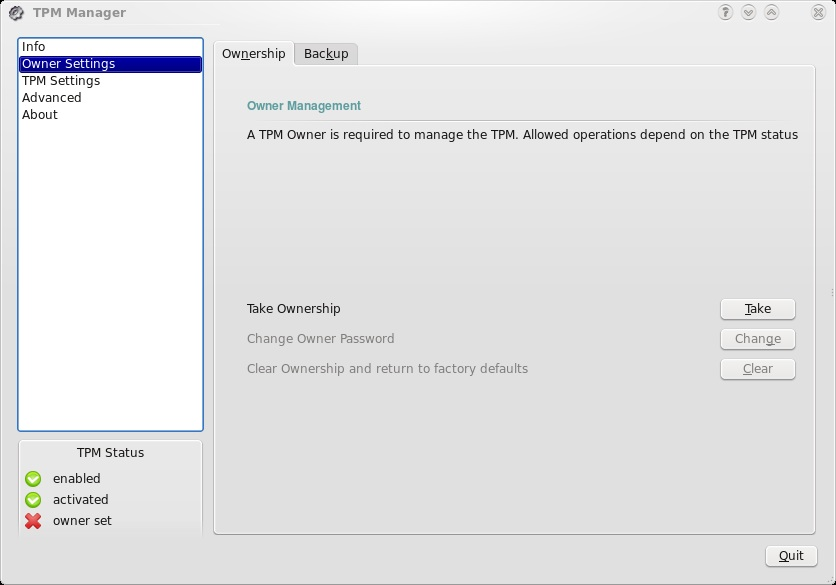
\includegraphics[width=0.8\textwidth]{images/tpmmanager_noowner.jpg}
   \caption{Take ownership}
\label{fig:take}
\end{figure}
\begin{figure}[h]
 \centering
   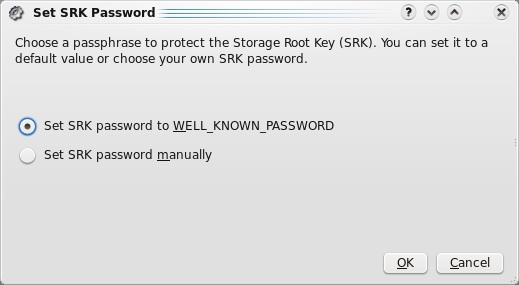
\includegraphics[width=0.6\textwidth]{images/tpmmanager_take_srk.jpg}
   \caption{Dialog for setting SRK}
\label{fig:srk}
\end{figure}
\begin{figure}[h]
 \centering
   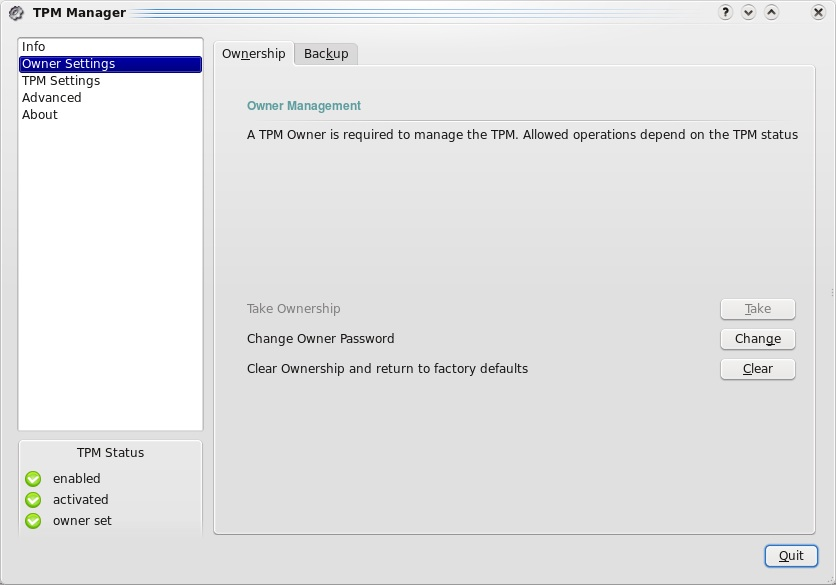
\includegraphics[width=0.8\textwidth]{images/tpmmanager_owner.jpg}
   \caption{After take ownership}
\label{fig:take2}
\end{figure}
\clearpage
\subsubsection{Backup tab} This functional area provides the possibility to create a new maintenance archive or to load an older archive into the TPM.

\subsection{TPM Settings} This functional area provides an interface to manage the TPM settings, such as Enable/Disable the TPM on ``Operational Modes'' tab or manage \AIK on the ``Identity'' tab, see bellow for more details. 
   \subsubsection{Operational Modes tab} The ``Deactivate`` button provides the ability to temporarily deactivate the TPM. If the TPM has an owner the button ''Enable``/''Disable`` allows to enable/disable the TPM, using the owner password. See \autoref{fig:disable} for a TPM status that has an owner and is enabled. Following the next steps you can disable the TPM:

\begin{itemize}
   \item Click in the left menu on the ''TPM Settings`` entry.
   \item Choose the ''Operational Modes`` tab
   \item Press ''Disable`` button
   \item Enter the owner password
   \item Confirm the next dialog if you really want to disable the TPM
   \item You will see that the TPM is actually disabled. See \autoref{fig:enable}
\end{itemize}

\begin{figure}[h]
 \centering
   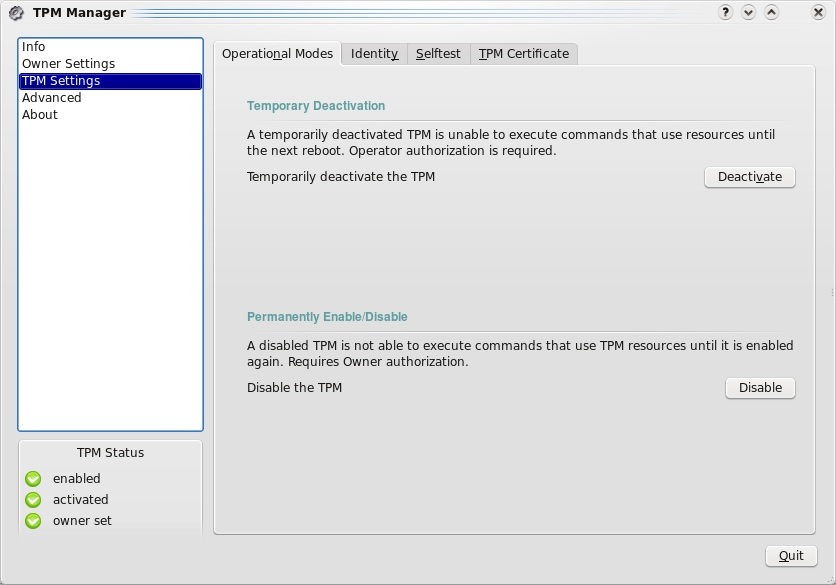
\includegraphics[width=0.8\textwidth]{images/tpmmanager_enabled.jpg}
   \caption{Status of an enabled TPM }
\label{fig:disable}
\end{figure}
\begin{figure}[h]
 \centering
   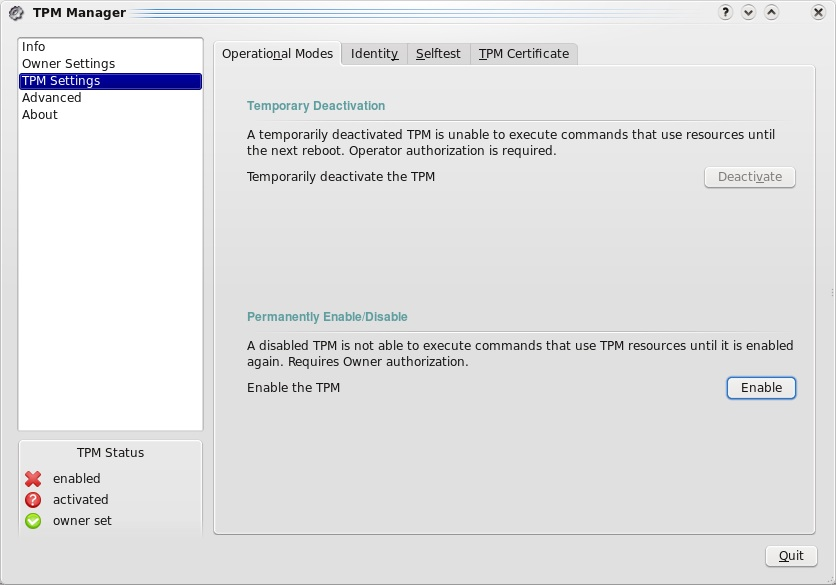
\includegraphics[width=0.8\textwidth]{images/tpmmanager_disabled.jpg}
   \caption{Status of the TPM after disabling}
\label{fig:enable}
\end{figure}
\clearpage

\subsubsection{Identitiy tab} This functional area provides management functions of the \EK. The functionalities ''Create`` and ''Restrict`` EK are not implemented yet. However, you can see the key information and save the public part of the EK to your PC. 
\subsubsection{Selftest tab} This tab allows you to perform the TPM selftest, a full test of each internal TPM function.
\subsubsection{TPM Certificate tab} Not implemented yet.

\subsection{Advanced} This section provides an interface to do some advanced TPM operations, such as disabling maintenance archive or deleting the Endorsement Key. Most functions of this section are not implemented yet.




% ------------------------------------------------------------------------
%\section{Open Issues}
%\begin{itemize}
%\item ...
%\end{itemize}

\end{document}
